\chapter{Linear classification}

\section{Theory}

In linear classification the decision surfaces are linear functions of the input vector $\mathbf{b}$. 
The decision surfaces are defined by D-1 dimensional hyperplane in the D dimensional input space.
the target of the classification is labelled in the target variable $\mathbf{t}$, using the target values to represent class labels. 
In the case of two-class problems, a single target variable can be represented by $t\in \lbrace 0,1\rbrace$ where $t = 1$ represents class $C_1$ and $t = 0$ represents class $C_2$.
If the is more than 2 classes $(K>2)$, then $\mathbf{t}$ is a vector of length K.
For Class $C_j$ the element $t_j$ takes value 1 and all other elements $t_k$ of $\mathbf{t}$ are zero.
In this project there are 3 different speakers, $K = 3$ then the target vector for class 3 be $\mathbf{t} = (0, 0, 1)^T$.
The value of $t_k$ can be interpreted as the probability of the given class being class $C_k$.
To assign each vector $\mathbf{x}$ with a specific class, a number of different approaches can used to classify.
One way is using a discriminant function, with a linear predictor $y(\mathbf{x},\mathbf{w})$ given by the parameter $\mathbf{w}$ and the input vector set $\mathbf{x}=(x_1,...,x_D)^T$, which is linear. 
The linear discriminant function in its simplest form

\begin{equation}
y(\mathbf{x}) = \mathbf{w}^T \mathbf{x}+w_0
\label{eq:lineDis}
\end{equation}

Where $w_0$ is the bias and $\mathbf{w}$ is the weight vector.
The decision boundary corresponds to $y(\mathbf{x})=constant$, and hence $\mathbf{w}^T \mathbf{x}+w_0 = constant$ therefore the decision boundary is a linear function.

The process to apply the linear classifier to the dataset, is described below. 
The result of the linear classifier is evaluated by applying a confusion matrix and calculating the accuracy. 
The linear classifier is applied to the training dataset, containing $N =??$ feature vectors $(\mathbf{x}_n)$ and the target vectors $(\mathbf{t}_n)$.
The vectors are on the form:
\begin{equation}
\mathbf{\tilde{X}}=\left[ \begin{array}{c}\mathbf{x}_1^T 1\\
\mathbf{x}_2^T 1\\
...\\ 
\mathbf{x}_n^T 1 \end{array} \right],
\;
\mathbf{T}=\left[ \begin{array}{c}
\mathbf{t}_1^T\\ 
\mathbf{t}_2^T\\ 
...\\
\mathbf{t}_n^T
\end{array} \right]
\label{eq:linearVectors}  
\end{equation} 

To determine the weight matrix $\tilde{\mathbf{W}}$:
\begin{equation}
\tilde{\mathbf{W}} = \tilde{\mathbf{X}}^\dagger \mathbf{T} \approx  (\tilde{\mathbf{X}}^T \tilde{\mathbf{X}}+\mathbf{I})^{-1} \tilde{\mathbf{X}}^T\mathbf{T}
\label{eq:weightVector}  
\end{equation}

The are a problem with the entity $\tilde{\mathbf{X}}^T \tilde{\mathbf{X}}$ having small eigenvalues, the solution is to add the identity matrix in the calculations of the pseudo inverse matrix $\tilde{\mathbf{X}}^\dagger$.
This is done as a regularization, which can be seen as a penalty for large values in $\tilde{\mathbf{W}}$.\\

When $\tilde{\mathbf{W}}$ is calculated from the training set, it is tested on the test dataset containing $N = ??$ feature vectors and their corresponding targets. 
The result of this equation
\begin{equation}
\mathbf{y}(\mathbf{x}) = \tilde{\mathbf{W}}^{T} \tilde{x},
\;
\tilde{x} = \left[\begin{array}{c}
\mathbf{x}\\ 1
\end{array} \right] 
\label{eq:Yclassifier}
\end{equation}
\fxnote{Er 1'erne ikke en søjle vector ved siden af x}
shows the most likely class for each of the given feature vectors. 
The resulting vector is placed in a vector $\mathbf{t}_{est}$, which contains the classification and ranges over the three classes ${1,2,3}$. show t estimate %\fixme

To evaluate the linear classifier, the confusion matrix is an ideal way of doing so.



\section{Method}
\fxnote{Indsæt metode afsnit. Evt med noget at det ovenfra}


\section{Results}
\subsection{Single digit:}

\begin{figure}[H]
\centering
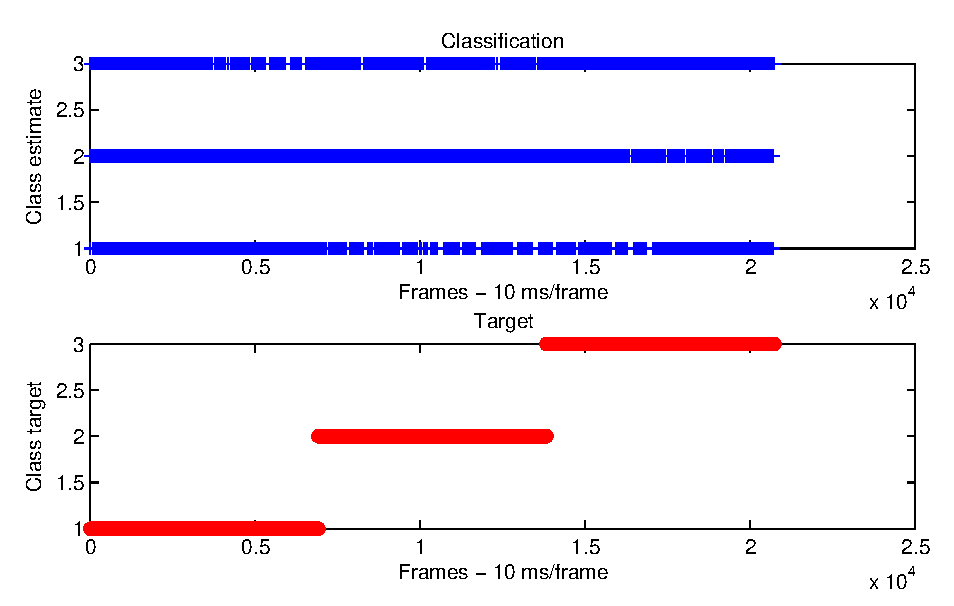
\includegraphics{Linear_1digit_8cent_3speak}
\caption{Results of using linear classifiers and single digit spoken}
\label{fig:Lin_fig_1}
\end{figure}

\begin{table}[H]                                                    
\centering                                                          
\begin{tabular}{|c|c|c|c|c|}                                        
\hline                                                              
  & Speaker Jacob & Speaker Mose & Speaker Simon & Precision [\%] \\
\hline                                                              
Estimate Jacob & 3169.0 & 830.0 & 1535.0 & 57.3 \\                  
\hline                                                              
Estimate Mose & 2163.0 & 3896.0 & 1818.0 & 49.5 \\                  
\hline                                                              
Estimate Simon & 1578.0 & 2184.0 & 3557.0 & 48.6 \\                 
\hline                                                              
Sensitivity [\%] & 45.9 & 56.4 & 51.5 & 51.2 \\                     
\hline                                                              
\end{tabular}                                                       
\caption{Confusion matrix - 1 digit}                                
\label{table:Lin_conf_1}                                            
\end{table}     
                   

\subsection{2 digits:}

\begin{figure}[H]
\centering
\includegraphics{Linear_2digit_8cent_3speak}
\caption{Results of using linear classifiers and two digits spoken}
\label{fig:Lin_fig_2}
\end{figure}

\begin{table}[H]                                                    
\centering                                                          
\begin{tabular}{|c|c|c|c|c|}                                        
\hline                                                              
  & Speaker Jacob & Speaker Mose & Speaker Simon & Precision [\%] \\
\hline                                                              
Estimate Jacob & 2041.0 & 557.0 & 699.0 & 61.9 \\                   
\hline                                                              
Estimate Mose & 562.0 & 1816.0 & 820.0 & 56.8 \\                    
\hline                                                              
Estimate Simon & 851.0 & 1081.0 & 1935.0 & 50.0 \\                  
\hline                                                              
Sensitivity [\%] & 59.1 & 52.6 & 56.0 & 55.9 \\                     
\hline                                                              
\end{tabular}                                                       
\caption{Confusion matrix - 2 digit}                                
\label{table:Lin_conf_2}                                            
\end{table}                                


\subsection{10 digits:}

\begin{figure}[H]
\centering
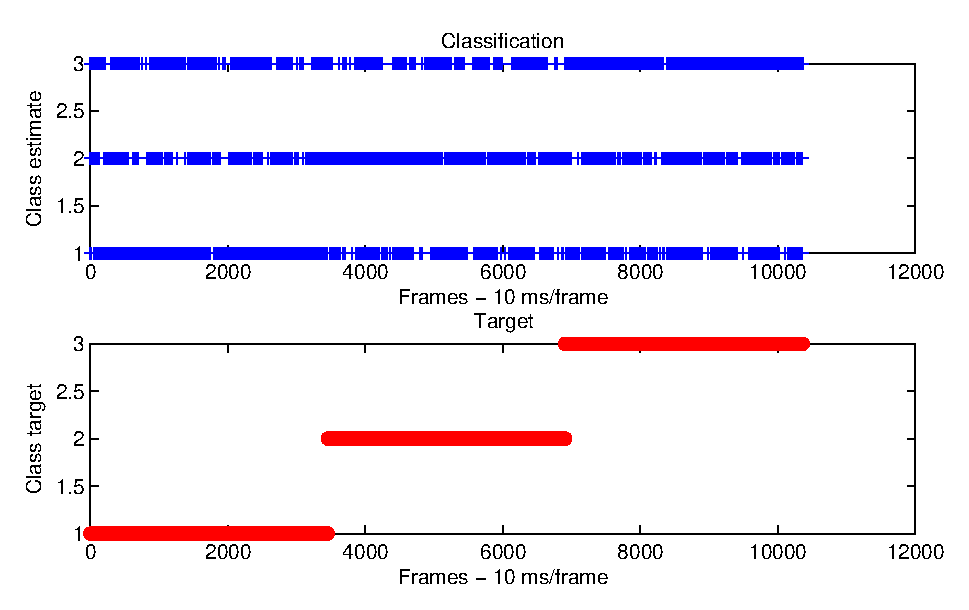
\includegraphics{Linear_10digit_8cent_3speak}
\caption{Results of using linear classifiers and ten digits spoken}
\label{fig:Lin_fig_2}
\end{figure}
\begin{table}[H]                                                    
\centering                                                          
\begin{tabular}{|c|c|c|c|c|}                                        
\hline                                                              
  & Speaker Jacob & Speaker Mose & Speaker Simon & Precision [\%] \\
\hline                                                              
Estimate Jacob & 2041.0 & 557.0 & 699.0 & 61.9 \\                   
\hline                                                              
Estimate Mose & 562.0 & 1816.0 & 820.0 & 56.8 \\                    
\hline                                                              
Estimate Simon & 851.0 & 1081.0 & 1935.0 & 50.0 \\                  
\hline                                                              
Sensitivity [\%] & 59.1 & 52.6 & 56.0 & 55.9 \\                     
\hline                                                              
\end{tabular}                                                       
\caption{Confusion matrix - 10 digits}                              
\label{table:Lin_conf_10}                                           
\end{table}                                                         


\section{Discussion}
\fxnote{Indsæt diskussion}









